

\documentclass[11pt, reqno]{article}   	% use "amsart" instead of "article" for AMSLaTeX format
\usepackage{my_packages}

\title{PCRTBP Invariant Manifolds}
\author{Shankar Kulumani}
\date{3 July 2017}							% Activate to display a given date or no date

\begin{document}
\maketitle
\subsection{Variational Integrator}\label{sec:discrete_var}
% description of variational integrator development
Geometric numerical integration deals with numerical integration methods which preserve the geometric properties of the flow of a differential equation, such as invaraint properties and symplecticity.
Variational integrators are constructed by discretizing Hamilton's principle rather than the continuous Euler-Lagrange equations~\cite{marsden2001}.
As a result, integrators developed in this manner have the desirable properties that they are symplectic and momentum preserving.
In addition, they exhibit improved energy behavior over long integration periods.
We present a short background on the variational principle for mechanical systems. 
We then develop a discrete approximation of the action integral and construct a variational integrator for the PCRTBP.

\subsection{Variational Principle}
Consider a continuous mechanical system described by the Lagrangian, \( L( q, \dot{q} ) \), for the generalized position, \( q\), and velocity, \( \dot{q} \).
In the standard approach of variational mechanics the action integral is formed by integrating the continuous Lagrangian along a path \( q(t) \) that the system follows from time \( t = 0 \) to \( t = T \)~\cite{greenwood1988}.
In the continuous time the action integral is defined as
\begin{align}\label{eq:action_integral}
        S = \int_{0}^T L\left( q, \dot{q}\right) \, dt \, .
\end{align}
Hamilton's principle states that the actual path followed by a holonomic system results in a stationary action integral with respect to path variations for fixed endpoints.
Taking the variation of~\cref{eq:action_integral} gives
\begin{align}\label{eq:var_principle}
        \delta S %&= \int_{0}^T \deriv{L}{q} \delta q + \deriv{L}{\dot{q}} \delta \dot{q} \, dt \\
                %&= \int_{0}^T \deriv{L}{q} \delta q - \frac{d}{dt} \left( \deriv{L}{\dot{q}}\right) \delta q \, dt - \left. \left[ \deriv{L}{\dot{q}} \delta q\right] \right|_0^T \\
        &= \int_{0}^T \deriv{L}{q} - \frac{d}{dt} \left( \deriv{L}{\dot{q}}     \right) \, dt \, ,
\end{align}
where we have used integration by parts and the conditions \( \delta q(0) = 0 \) and \( \delta q(T) = 0\).
For Hamilton's principle to be valid for all admissible variations \( \delta q \), the integrand of~\cref{eq:var_principle} must be zero for all \( t\), giving the continuous Euler-Lagrange Equations~\cite{lanczos1970}.
\begin{align}\label{eq:euler-lagrange}
        0 = \deriv{L}{q} - \frac{d}{dt} \left( \deriv{L}{\dot{q}} \right) \, .
\end{align}
Hamilton's equations are derivable through the use of the Legendre transformation which is a mapping \( \left( q, \dot{q},t\right) \rightarrow \left(q, p, t \right) \) where \( p_i\) is the generalized momenta.
\begin{align}\label{eq:legendre_transform}
        p_i = \deriv{L}{\dot{q}_i} \, .
\end{align}
In the continuous time case the Hamiltonian is defined as
\begin{align}\label{eq:hamiltonian}
        H &= \sum_{i = 1}^n p_i \dot{q}_i - L \left( q,\dot{q}, t \right) \, .
\end{align}
Applying~\cref{eq:legendre_transform} and taking the variation of~\cref{eq:hamiltonian} allows us to derive the equations of motion in Hamiltonian form
\begin{subequations}\label{eq:hamilton_eq}
\begin{align}
        \dot{q}_i &= \deriv{H}{p_i} \, ,\\
        \dot{p}_i &= - \deriv{H}{q_i} \, , \\
        \deriv{L}{t} &= -\deriv{H}{t} \, .
\end{align}
\end{subequations}
Both~\cref{eq:euler-lagrange,eq:hamilton_eq} result in equations of motion for the mechanical system and are equivalent via the Legendre transform.
\Cref{eq:euler-lagrange} results in \( n \) second order differential equations while~\cref{eq:hamilton_eq} results in \( 2n \) first order differential equations.
\subsection{Discrete Variational Mechanics}
A discrete analogue of Hamilton's principle and the action integral is formed.
Rather than taking a position, \( q \), and velocity, \( \dot{q} \), consider two positions \( q_0 \) and \( q_1 \) and a fixed time step \( h \in \R \).
The two positions are points on the curve \( q(t) \) such that \( q_0 \approx q(0) \) and \( q_1 \approx q(h) \).
A discrete time Lagrangian \( L_d( q_0, q_1) \) is formed which approximates the action integral between \( q_0 \) and \( q_1 \) as 
\begin{align}\label{eq:discrete_lagrangian_gen}
        L_d\left( q_0 , q_1 \right) \approx \int_{0}^{h} L \left( q , \dot{q} \right) \, dt \, .
\end{align}
Since~\cref{eq:discrete_lagrangian_gen} is calculated as a numerical integral, an appropriate quadrature rule is required.
There are multiple possible methods one can use to approximate the integral in~\cref{eq:discrete_lagrangian_gen}.
An appropriate approximation rule is determined based on the ease of implementation and accuracy desired.
\begin{table}[htbp]
\caption{Selected Quadrature Rules\label{tab:quadrature}}
\begin{center}
\begin{tabular}{l|l}Rectangle & \( L_d(q_0,q_1) =L(q_0,\frac{q_1-q_0}{h}) h \)  \\ \hline
Midpoint & \( L_d(q_0,q_1) = L(\frac{q_0 + q_1}{2},\frac{q_1 - q_0}{h}) h \) \\ \hline
Trapezoidal & \( L_d(q_0, q_1) = \frac{1}{2} \left[ L(q_0, \frac{q_1 - q_0}{h} ) + L(q_1, \frac{q_1 - q_0 }{h} )\right] h \)
\end{tabular} 
\end{center}
\end{table}
\Cref{tab:quadrature} shows several possible approximation rules that are typically applied.
The rectangle rule is a first order accurate method and offers a straightforward implementation.
The midpoint and trapezoidal rules are both second order accurate methods. 
However, the midpoint rule results in an implicit form which adds further complexity to the equations of motion.
%In this work, the trapezoidal approximation is applied to the PCRTBP.

Once an appropriate discrete Lagrangian is formed a discrete action sum is formed as the discrete analogue of~\cref{eq:action_integral}
\begin{align}\label{eq:action_sum}
        S_d = \sum_{k=0}^{N-1} L_d(q_k, q_{k+1}) \, .
\end{align}
Once again a discrete version of Hamilton's principle is applied to~\cref{eq:action_sum}.
This yields a discrete time counterpart to~\cref{eq:var_principle} as
\begin{align}\label{eq:dis_var_principle}
        \delta S_d %&= \sum_{k=0}^{N-1} \deriv{L_d(q_k, q_{k+1})}{q_k} \delta q_k + \deriv{L_d(q_k, q_{k+1})}{q_{k+1}} \delta q_{k+1} \\
        &= \sum_{k=1}^{N-1} \bracket{ \deriv{L_d(q_k, q_{k+1})}{q_k} + \deriv{L_d(q_{k-1}, q_k)}{q_{k+1}}} \delta q_k \, .
\end{align}

For the discrete action sum to be stationary with respect to all admissible path variations, with fixed endpoints, the discrete Euler-Lagrange equations must be satisfied for \( k = 1, \cdots, N-1 \) resulting in
\begin{align}\label{eq:discrete_euler-lagrange}
        0 = \deriv{L_d(q_k, q_{k+1})}{q_k} + \deriv{L_d(q_{k-1}, q_k)}{q_{k+1}} \, .
\end{align}
A discrete version of the Legendre transformation, referred to as a discrete fiber derivative, results in the equivalent Hamiltonian form expression.
The discrete fiber derivative is given as 
\begin{subequations}\label{eq:discrete_legendre}
\begin{align}
        p_k &= \deriv{L_d(q_{k-1},q_k)}{q_{k+1}} = - \deriv{L_d(q_k, q_{k+1})}{q_k} \, ,\\
        p_{k+1} &= \deriv{L_d(q_k, q_{k+1})}{q_{k+1}} \, .
\end{align}
\end{subequations}
This yields a discrete Hamiltonian map \( (q_k, p_k) \to (q_{k+1}, p_{k+1}) \).
A more extensive development of variational integrators can be found in~\cite{marsden2001}.

\subsection{Discrete Equations of Motion}
The discrete equations of motion for the PCRTBP are derived by choosing an appropriate quadrature rule to discretize the Lagrangian in~\cref{eq:lagrangian}. 
In this work, the trapezoidal approximation is applied.
The trapezoid rule allows for an explicit second order accurate approximation.
The discrete Lagrangian is given by
\begin{align}\label{eq:discrete_lagrangian}
        L_d = &\frac{h}{2} \left( \frac{1}{2} \bracket{\left(  \frac{\xkp - \xk}{h} -\yk \right)^2 + \left( \frac{\ykp - \yk}{h} + \xk \right)^2} + \frac{1 - \mu}{r_{1_k}} + \frac{\mu}{r_{2_k}} \right. \nonumber \\ 
                & + \left. \frac{1}{2} \bracket{\left(  \frac{\xkp - \xk}{h} -\ykp \right)^2 + \left( \frac{\ykp - \yk}{h} + \xkp \right)^2} + \frac{1-\mu}{r_{1_{k+1}}} + \frac{\mu}{r_{2_{k+1}}}  \right) \, .
\end{align}
Applying a discrete version of the Lagrange-d'Alembert principle allows for inclusion of an external control force on the system~\cite{marsden2001}.
Using~\cref{eq:discrete_legendre,eq:discrete_lagrangian} and some manipulation, the equations of motion are given by
\begin{subequations}\label{eq:discrete_eoms}
\begin{align}
        \xkp &= \frac{1}{1+ h^2} \bracket{h \dot{x}_k + h^2 \dot{y}_k  + \xk \parenth{1+ \frac{3h^2}{2}} + \frac{h^3}{2} \yk - \frac{h^3}{2} U_{y_k} - \frac{h^2}{2} U_{x_k} } \label{eq:xkp} \, ,\\
        \ykp &= h \dot{y}_k + h \xk - h \xkp + \yk + \frac{h^2 \yk}{2} - \frac{h^2 }{2} U_{y_k} \label{eq:ykp} \, ,\\
        \dot{x}_{k+1} &= \dot{x}_k - 2 \yk + 2 \ykp + \frac{h}{2} \parenth{\xkp + \xk} - \frac{h}{2} U_{\xkp} - \frac{h}{2} U_{\xk} + h u_x \label{eq:xdotkp}\, ,\\
        \dot{y}_{k+1} &= \dot{y}_{k} + 2 \xk - 2 \xkp + \frac{h}{2} \parenth{\ykp + \yk} - \frac{h}{2} U_{\ykp} - \frac{h}{2} U_{\yk} + h u_y \label{eq:ydotkp} \, .
\end{align}
\end{subequations}
The discrete equations of motion are given in the Lagrangian form after applying the discrete fiber derivative from~\cref{eq:discrete_legendre} as \( p_{\xk} = \dot{x}_k - \yk \) and \( p_{\yk} = \dot{y}_k + \xk \).
The state is defined as \( \vecbf{x}_k = \begin{bmatrix} \xk & \yk & \dot{x}_k & \dot{y}_k \end{bmatrix}^T\) and the control input is \( \vecbf{u} = \begin{bmatrix} u_x & u_y \end{bmatrix}^T \).
This results in a discrete update map \( f_k: \vecbf{x}_k \to \vecbf{x}_{k+1} \) which preserves the same properties of the continuous-time dynamics in~\cref{eqn:cont_dyn} such as invariants, symplecticity, and the configuration manifold.
The discrete potential gradients are given by
\begin{subequations}\label{eq:discrete_potential_grad}
\begin{align}
        U_{\xk} &= \frac{\parenth{1 -\mu} \parenth{\xk + \mu}}{\distonek^3} + \frac{ \mu \parenth{\xk -1 + \mu}}{\disttwok^3} \label{eq:Uxk} \, ,\\
        U_{\yk} &= \frac{\parenth{1 -\mu} \yk}{\disttwok^3} + \frac{ \mu \yk}{\disttwok^3} \label{eq:Uyk} \, ,\\
        U_{\xkp} &= \frac{\parenth{1 -\mu} \parenth{\xkp + \mu}}{\distonekp^3} + \frac{ \mu \parenth{\xkp -1 + \mu}}{\disttwokp^3} \label{eq:Uxkp}\, ,\\
        U_{\ykp} &= \frac{\parenth{1 -\mu} \ykp}{\distonekp^3} + \frac{ \mu \ykp}{\disttwokp^3} \label{eq:Uykp} \, .
\end{align}     
\end{subequations}
The distances to each primary are defined as
\begin{subequations}\label{eq:discrete_distance}
\begin{align}
        \distonek &= \sqrt{\left( \xk + \mu\right)^2 + \yk^2} \label{eq:distonek}\, ,\\
        \disttwok &= \sqrt{\left( \xk - 1 + \mu\right)^2 + \yk^2} \label{eq:disttwok}\, ,\\
        \distonekp &= \sqrt{\left( \xkp + \mu\right)^2 + \ykp^2} \label{eq:distonekp}\, ,\\
        \disttwokp &= \sqrt{\left( \xkp - 1 + \mu\right)^2 + \ykp^2} \label{eq:disttwokp} \, .
\end{align}
\end{subequations}
Care must be taken during the implementation of~\cref{eq:discrete_eoms}.
As~\cref{eq:discrete_potential_grad,eq:discrete_distance} are defined at both step \( k \) and \( k+1 \) they must be evaluated at both time instances.
\Cref{eq:discrete_eoms} is implemented by first defining an initial state \( \vecbf{x}_k \) and control \( \vecbf{u}_k \).
The distances and gravitational potential at step \( k \) are evaluated from~\cref{eq:distonek,eq:disttwok,eq:Uxk,eq:Uyk}.
The discrete update steps in~\cref{eq:xkp,eq:ykp} are evaluated to generate \( \xkp \) and \( \ykp\).
Next, the distances and gravitational potential at step \( k+1 \) are evaluated from~\cref{eq:distonekp,eq:disttwokp,eq:Uxkp,eq:Uykp}. 
Finally, the update steps in~\cref{eq:xdotkp,eq:ydotkp} are evaluated.
This results in the complete discrete update map \( \vecbf{x}_k \to \vecbf{x}_{k+1} \) given \( \vecbf{u}_k \).
\subsection{Numerical Example}\label{sec:variational_example}
\begin{figure} 
        \centering 
        \begin{subfigure}[h]{0.5\textwidth} 
                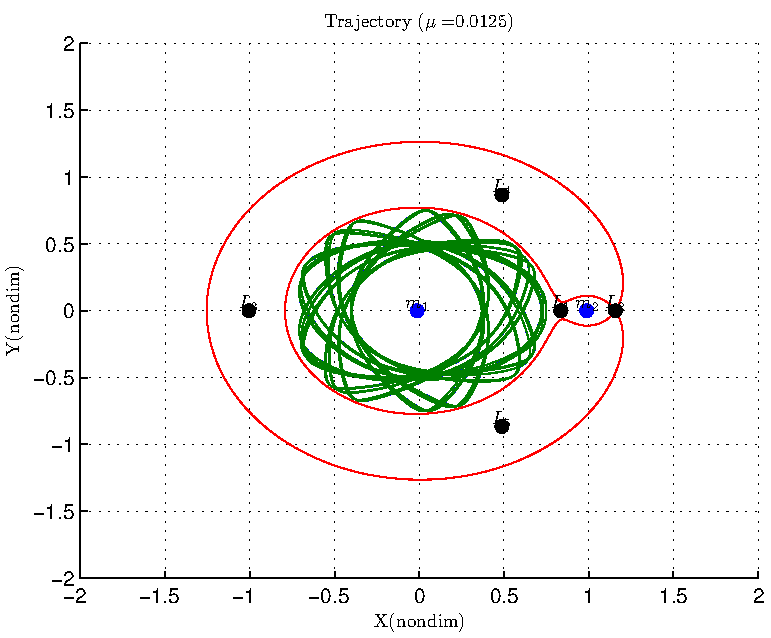
\includegraphics[width=\textwidth]{trajectory} 
                \caption{Trajectory comparison} \label{fig:compare_trajectory} 
        \end{subfigure}~ %add desired spacing between images, e. g. ~, \quad, \qquad, \hfill etc. %(or a blank line to force the subfigure onto a new line) 
%       \begin{subfigure}[htbp]{0.3\textwidth} 
%               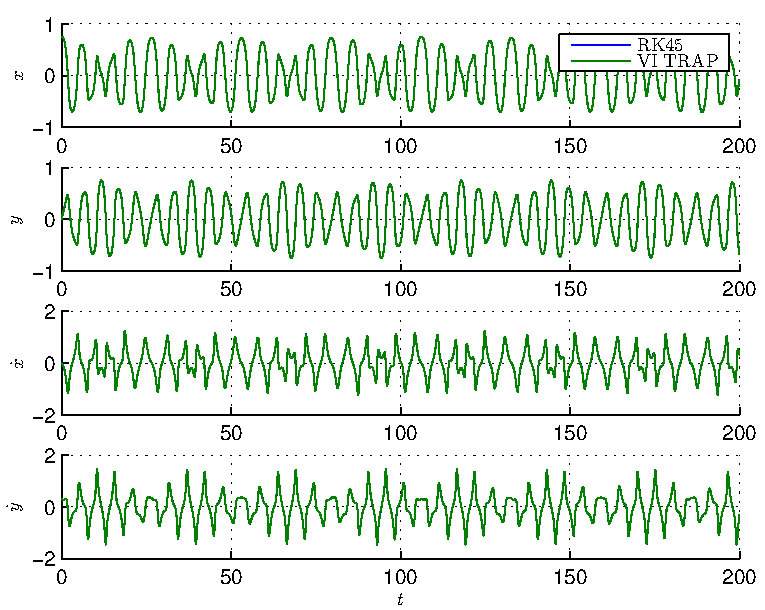
\includegraphics[width=\textwidth]{components} 
%               \caption{State \( \parenth{x , y, \dot{x}, \dot{y}}\)} \label{fig:compare_components} 
%       \end{subfigure} ~ %add desired spacing between images, e. g. ~, \quad, \qquad, \hfill etc. %(or a blank line to force the subfigure onto a new line) 
        \begin{subfigure}[htbp]{0.5\textwidth} 
                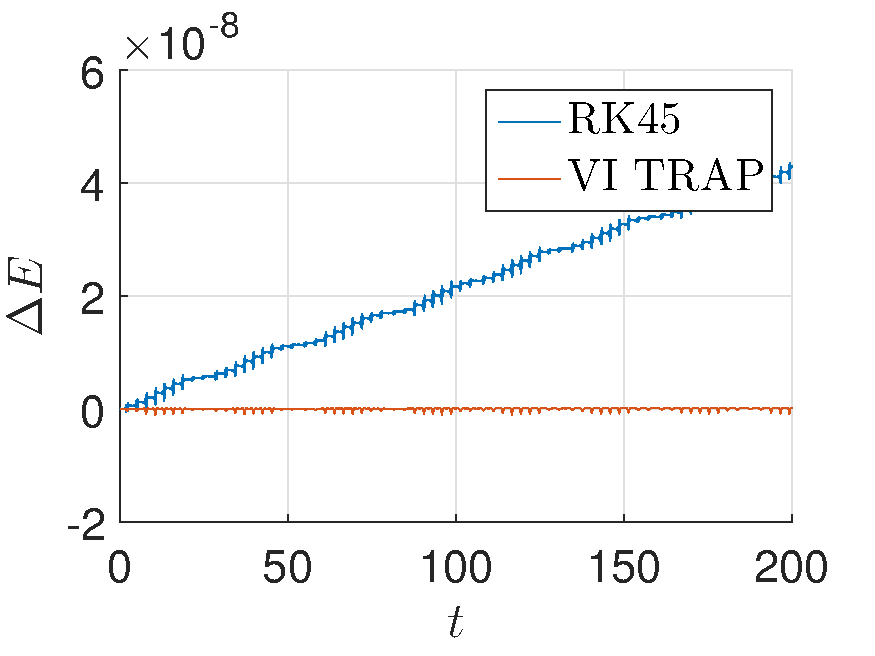
\includegraphics[width=\textwidth]{energy} 
                \caption{Jacobi Integral comparison} \label{fig:compare_energy} 
        \end{subfigure} 
        \caption{Integrator Comparison}
        \label{fig:integrator_compare} 
\end{figure}
A simulation comparing the variational integrator to a conventional Runge-Kutta method is given in~\cref{fig:integrator_compare}.
A particle is simulated from an initial condition of \( \vecbf{x}_0 = \begin{bmatrix} 0.75 & 0 & 0 & 0.2883\end{bmatrix}^T \) for \( t_f = 200 \approx 15\) years in the Earth-Moon system.
The variational integrator uses a step size of \SI{47.22}{\second} while the Runge-Kutta method uses a variable step size implemented via ODE45 in Matlab.
\Cref{fig:compare_trajectory} shows the trajectory of the spacecraft in the rotating reference frame for both integration schemes.
Both integration schemes result in trajectories that are initially nearly identical.
The discrete equations of motion are an accurate approximation for the continuous dynamics as they closely match the solution of ODE45 over the initial portion of the simulation.
However, as time progresses the trajectories begin to diverge due to the differences in system energy.
\Cref{fig:compare_energy} shows the evolution of the Jacobi integral.
The variational integrator exhibits a bounded behavior about the initial energy with a mean variation of \num{4.2522e-20}.
However, the conventional Runge-Kutta method demonstrates a clear energy drift of \num{4.2814e-8}. 
Over long simulation horizons or with the addition of small control inputs this poor energy behavior limits the applicability of conventional techniques.
\section*{Appendix B: Gauss Jordan Elimination}\label{sec:costate_gauss_jordan}
The costate equations of motion are given by~\cref{eq:costate_eom} and repeated here as
\begin{align}\label{eq:costate_eom_transpose}
        \begin{bmatrix} 
                \fonex & \ftwox & \fthreex & \ffourx \\
                \foney & \ftwoy & \fthreey & \ffoury \\
                \fonexd & \ftwoxd & \fthreexd & \ffourxd \\
                \foneyd & \ftwoyd & \fthreeyd & \ffouryd
        \end{bmatrix}
        \begin{bmatrix} \lambda_{\xkp} \\ \lambda_{\ykp} \\ \lambda_{\xdotkp} \\ \lambda_{\ydotkp} \end{bmatrix}
        =
        \begin{bmatrix} \lambda_{\xk} \\ \lambda_{\yk} \\ \lambda_{\xdotk} \\ \lambda_{\ydotk} \end{bmatrix} \, .
\end{align}
To determine the discrete update map \( \lambda_k \to \lambda_{k+1}\) the inverse of the Jacobian matrix is required.
In order to avoid the need of an explicit inversion a Gauss Jordan method is implemented.
To begin, several terms are defined which are required to carry out the row operations and are defined as
\begin{subequations}\label{eq:ref_scale}
\begin{align}
        a &= -\frac{\foney}{\fonex} \, ,\\
        b &= -\frac{\fonexd}{\fonex} \, , \\
        c &= -\frac{\foneyd}{\fonex} \, ,\\
        e &= -\frac{\ftwoxd + b \ftwox}{\ftwoy + a \ftwox} \, ,\\
        f &= -\frac{\ftwoyd + c \ftwox}{\ftwoy + a \ftwox} \, ,\\
        g &= -\frac{\fthreeyd + c \fthreex + f \parenth{\fthreey + a \fthreex}}{\fthreexd + b \fthreex + e \parenth{\fthreey + a \fthreex}}\, .
\end{align}
\end{subequations}
\Cref{eq:costate_eom_transpose} is transformed to row echelon form using elementary row operations and is defined as
\begin{align}\label{eq:costate_ref}
        \begin{bmatrix} 
                \alpha_{11} & \alpha_{12} & \alpha_{13} & \alpha_{14} \\
                0 & \alpha_{22} & \alpha_{23} & \alpha_{24} \\
                0 & 0 & \alpha_{33} & \alpha_{34} \\
                0 & 0 & 0 & \alpha_{44}
        \end{bmatrix}
        \begin{bmatrix} \lambda_{\xkp} \\ \lambda_{\ykp} \\ \lambda_{\xdotkp} \\ \lambda_{\ydotkp} \end{bmatrix}
        =
        \begin{bmatrix} \beta_1 \\ \beta_2 \\ \beta_3 \\ \beta_4 \end{bmatrix} \, ,
\end{align}
where the terms \( \alpha_{ij} \) and \( \beta_{i} \) are defined as follows
\begin{subequations}
\begin{align}
        \alpha_{11} &= \fonex \, ,\\
        \alpha_{12} &= \ftwox \, ,\\
        \alpha_{13} &= \fthreex \, ,\\
        \alpha_{14} &= \ffourx \, ,\\
        \alpha_{22} &= \ftwoy + a \ftwox \, ,\\
        \alpha_{23} &= \fthreey + a\fthreex \, ,\\
        \alpha_{24} &= \ffoury + a \ffourx \, ,\\
        \alpha_{33} &= \fthreexd + b \fthreex + e \parenth{\fthreey + a \fthreex}\, ,\\
        \alpha_{34} &= \ffourxd + b \ffourx + e \parenth{\ffoury + a \ffourx} \, ,\\
        \alpha_{44} &= \ffouryd + c \ffourx + f \parenth{\ffoury + a \ffourx} + g \parenth{\ffourxd + b \ffourx + e \parenth{\ffoury + a \ffourx}} \, ,\\
        \beta_1 &= \lambda_{\xk} \, ,\\
        \beta_2 &= \lambda_{\yk} + a \lambda_{\xk} \, ,\\
        \beta_3 &= \lambda_{\xdotk} + b \lambda_{\xk} + e \parenth{\lambda_{\yk} + a \lambda_{\xk}} \, ,\\
        \beta_4 &= \lambda_{\ydotk} + c \lambda_{\xk} + f \parenth{\lambda_{\yk}+a \lambda_{\xk}} + g \parenth{\lambda_{\xdotk} + b \lambda_{\xk} + e \parenth{\lambda_{\yk} + a \lambda_{\xk}}} \, .
\end{align}
\end{subequations}
Finally, backsubstituion is used to determine explicit equations for the discrete update map \( \vecbf{\lambda}_k \to \vecbf{\lambda}_{k+1} \) which is defined as
\begin{subequations}\label{eq:costate_update}
\begin{align}
        \lambda_{\ydotkp} &= \frac{\beta_4}{\alpha_{44}} \, ,\\
        \lambda_{\xdotkp} &= \frac{\beta_3}{\alpha_{33}} - \frac{\alpha_{34}}{\alpha_{33}} \lambda_{\ydotkp} \, ,\\
        \lambda_{\ykp} &= \frac{\beta_2}{\alpha_22} - \frac{\alpha_{33}}{\alpha_{22}}\lambda_{\xdotkp} - \frac{\alpha_{24}}{\alpha_{22}} \lambda_{\ydotkp} \, ,\\
        \lambda_{\xkp} &= \frac{\beta_1}{\alpha_{11}} - \frac{\alpha_{12}}{\alpha_{11}} \lambda_{\ykp} - \frac{\alpha_{13}}{\alpha_{11}} \lambda_{\xdotkp} - \frac{\alpha_{14}}{\alpha_{11}} \lambda_{\ydotkp} \, .
\end{align}
\end{subequations}
%Once again, these equations exhibit a cascade type relationship. 
%As as result any errors will compound and tend to accumulate most prevalently in \( \lambda_{\xkp} \).


\bibliographystyle{abbrv}
%\bibliography{../../../../docs/technical_papers/bibtex/library}
\bibliography{library}
\end{document}  
